\documentclass{article}
\usepackage{amsmath, amssymb, cite, algorithmic, url, braket}
\usepackage{graphicx}
\usepackage{pythonhighlight}
\usepackage[margin=1.5cm]{geometry}
\usepackage[title]{appendix}
\usepackage{subfigure}
\usepackage{listings}
\usepackage{booktabs}

\graphicspath{{../pic/}}
\lstset{
language=[ANSI]{C},
showtabs=true,
tab=,
tabsize=2,
basicstyle=\ttfamily\footnotesize,%\setstretch{.5},
stringstyle=\color{stringcolour},
showstringspaces=false,
alsoletter={1234567890},
otherkeywords={\%, \}, \{, \&, \|},
keywordstyle=\color{keywordcolour}\bfseries,
upquote=true,
morecomment=[s]{/*}{*/},
commentstyle=\color{commentcolour}\slshape,
literate=*%
{=}{{\literatecolour=}}{1}%
{-}{{\literatecolour-}}{1}%
{+}{{\literatecolour+}}{1}%
{*}{{\literatecolour*}}{1}%
{!}{{\literatecolour!}}{1}%
{[}{{\literatecolour[}}{1}%
{]}{{\literatecolour]}}{1}%
{<}{{\literatecolour<}}{1}%
{>}{{\literatecolour>}}{1}%
% {>>>}{\pythonprompt}{3}%
,%
frame=trbl,
rulecolor=\color{black!40},
backgroundcolor=\color{white},
breakindent=.5\textwidth,frame=single,breaklines=true
}

\begin{document}
\title{DSP Homework 08}
\author{Xu, Minhuan}
\maketitle
\tableofcontents
\begin{abstract}
\subsubsection*{Videos}
After summing up the videos, I learned more about the stretch robots in Boston Dynamics.
\subsubsection*{Comparison Between Two Sampling Methods}
First, I found out all aspects I can come out to compare the two sampling methods.

Second, I used an example to find out the relationship between the sampling period $T$ and the order of reconstructed signal $\hat{x}(t)$ in Wan Sampling Method.
\subsubsection*{USB Hubs and My Proposal about it}


\end{abstract}

\section{Videos}
\subsection{Boston Dynamics}
This video introduced the robots in Boston Dynamics briefly and mainly discussed about why somebody says that those robots can make soldiers obsolete. The robots' reliability, ruggedness, and most important, intelligence make that sound reasonable.

\subsubsection{Types of Robots in Boston Dynamics}

The robots in Boston Dynamics have 3 types, see the list below.
\begin{enumerate}
	\item[-] Automatic Robots: These robots must have inputs from human, which means they are just the extension of human arms and legs.
	\item[-] Automated Robots: These robots can have their own decision when they are facing a judgement which decides what they should do next. That kind of decision are in fact made by the program written by people in advance.
	\item[-] Autonomous Robots: These robots have the ability of not only making decisions but learning how to make decisions. They have more intelligence.
\end{enumerate}

However, if somebody wants robots to work like soldiers, this person means that the robots can complete a whole mission all by the robots themselves. To make this situation come true, there must be a synergy between mechanical parts and AI-powered programmed brain. Obviously, among those robots, only Autonomous Robots will have the change to replace the soldiers.

\subsubsection{Pros and Cons of Using Robots in the Military}

Also, we can know from the video what advantages and disadvantages those military concept robots have.
\begin{enumerate}
	\item[-] Advantages: No human will die in war; Adjusting to severe environment easily,
	\item[-] Disadvantages: vulnerable to hacking; AI out of control; moral issues like people who have access to the technology oppress those who don't.
\end{enumerate}

\subsection{Bone Density}
\subsubsection{How Our Body Change Bone Density}
The bones are made of some compact bone tissues outside and some spongy bone tissues inside. There are two kind of cells in spongy bone tissues, and one form new bone tissues, and the other absorb the old bone tissues. With the help of these two cells, the inside spongy bone tissues are able to adapt the architecture to the environment. 

\subsubsection{How We Can Raise Bone Density}
In this video, they said that once pushing force and pulling force are applied to bones, the bone will let cells produce more bone tissues to raise the bone density, vice versa. Therefore, the more force applied on the bone continuously, the more density bones will have. What's more, almost every kind of exercises we usually do works in that way. In one word, exercise strengthen our bones.

\subsection{My Thoughts}
Having watched the video about the military application of the Boston Dynamics, I am rather impressed by stretch, the warehouse logistics robots. They are smart that they can build up a assembly line all by themselves, and can use the arm to lift things and drop them. I can imagine its universal usage in the warehouse, classifying, rearrangement, pack up, and so on, what's important, it can work 24 hours. This completely fits my vision of life in the future. 

There's one thing I want to say, after watching other videos about the stretch, I found that the structure those robots use to lift and drop things, are a matrix of sucking discs. The problem is how can they handle the situation that the items that are not flat enough like the luggage boxes. It is not difficult for me to find one kind of things called sponge sucker, that thing can fit the surface first, and pump the air out, so that it can handle things that are not flat.

\section{Comparison Between Two Sampling Methods}

\subsection{Local Adaptivity}
We can know from the class that the reconstructed function of the wan Sampling Method usually be like
\begin{equation}
	\hat{x}(t) = x(nT) + x'(nT)(t - nT) \quad T \in [n - \frac12, n + \frac12)
	\label{eq:WanReconstruct}
\end{equation}
Therefore, a certain time $\hat{x}(t)$ can be expressed only using near sampling points.

But, in the Shannon/Nyquist Sampling Method, we have derived the reconstructed function many times and that is
\begin{equation}
	x(t) = \sum_{n = - \infty}^{\infty} x(nT) \cdot sinc(\frac{t - nT}{T})
\end{equation}
That means for a certain point $t_0$ we have 
\begin{equation}
	x(t_0) = \sum_{n = - \infty}^{\infty} x(nT) \cdot \mathrm{sinc}(\frac{t_0 - nT}{T})
	\label{eq:SN-Recon}
\end{equation}
and this specific value is associated with all sampling points.

Therefore, if the receiver got a piece of signal from the sender, it's hard to determine the sampling rate in advance in Shannon/Nyquist Sampling Method. However, in Wan Sampling Method we can use (\ref{eq:WanReconstruct}) to sample this little piece of signal.

\subsection{Circuits}
In Shannon/Nyquist Sampling Method, we need a filter which the cut-off frequency $f_c$ should be carefully chosen. Since the ideal LPF is not realizable, so engineers always use raised-cosine filter or root-raised-cosine filter to replace the ideal LPF. We have only learnt the analytical expressions of these two filters in The Principles of Communication and to implement it is difficult.

In Wan Sampling Method, see (\ref{eq:WanReconstruct}), mathematical methods we must use are just summation, multiple, differential calculus. In Analog Circuit, it is easy to do the plus, multiple, differential calculus using the operational amplifier.

\subsection{Flexible Error}
In Shannon/Nyquist Sampling Method, if we have determined the sampling rate in advance, the error is not predictable when the frequency of the signal is beyond the maximum frequency of Shannon/Nyquist Sampling Method.

In Wan Sampling Method, see subsection.\ref{wanSampling}, no matter what signal the receiver get, as long as we know the order of the reconstructed signal take, we can always find the maximum of the error. Moreover, if we take different order of the reconstructed signal,


\subsection{Flexible Bandwidth}
In Shannon/Nyquist Sampling Method, even there's only a little piece of the signal are relatively high-frequency, the sampling rate still should be set to the twice of the maximum frequency, otherwise there will be unpredictable error in the reconstructed function.

In Wan Sampling Method, because the reconstructed function $x(t)$ are only associated values within the interval of $[n - \frac12, n + \frac12)$. The signal bandwidth can be variable, which means we can choose wide-band channel when signal are wide-band, and choose narrow-band channel when signal are narrow band.

\subsection{My Understanding of Wan Sampling Method}
\label{wanSampling}

The Taylor Theorem is expressed as below.
$$
f(x) = \sum_{i = 0}^{N} ~ \frac{f^{(i)}(x_0)}{i!} ~ (x - x_0)^i + R_N(x)
$$

Applying to our signal $x(t)$, we can make $x_0 = nT, N = 2$ here and get the equation below. In this case, we assume that the value of $R_2(t)$ here is small enough compared with $\frac{x''(t_0)}{2}(x - t_0)^2$, so just ignore it.
\begin{equation}
	x(t) = x(nT) + x'(nT)(x - nT) + \frac{x''(t_0)}{2}(x - t_0)^2
\end{equation}


What exactly we get after sampling is only the values of $x(nT)$, but it is easy to do derivation. Therefore, using simple circuit, we know the values of $x'(nT),\,x''(nT),\,x'''(nT),\,\cdots$

So, the reconstructed signal $\hat{x}(t)$ can be expressed as
\begin{equation}
	x(t) = \overbrace{x(nT) + x'(nT)(x - nT)}^{\hat{x}(t)} + \frac{x''(t_0)}{2}(x - t_0)^2
\end{equation}
but also as
\begin{equation}
	x(t) = \overbrace{x(nT)}^{\hat{x}(t)} + x'(nT)(x - nT)
\end{equation}
The difference of the above two lies on the error of the reconstructed signal. It time to do the quantitative analysis, we assume that
\begin{equation}
	\begin{aligned}
		&|\hat{x}(t) - x(t)| &< \epsilon \\
		&|x^{(n)}(t)|  &< \eta_n \\ 
		&|x - nT|^n &< \frac{T}{2}
	\end{aligned}
\end{equation}
So, to ensure the accuracy, we need to make the sampling period $T$ satisfy the equations below.

\begin{equation}
	T < 2 \, \sqrt[n]{\frac{n! \,  \epsilon}{\eta_n}}
\end{equation}

About the value of $T$, I plotted a signal of $\cos(8t) + \sin(5t)\cos(2t)$ and the corresponding sampling period $T' = 2 \, \sqrt[n]{\frac{n!}{\eta_n}}$ ($\epsilon$ are ignored only to see the monotonicity of T about n), see Fig.~\ref{fig:maxes}.

\begin{figure}[!h]
	\centering
	\subfigure[Original Signal]{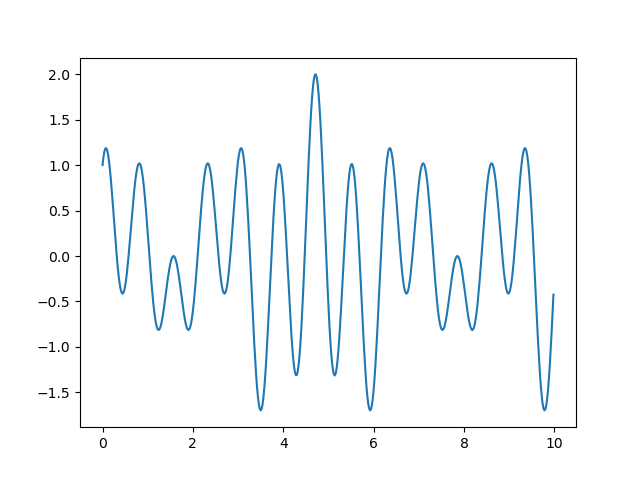
\includegraphics[height=2 in]{../pic/signal.png}}
	\hspace{0 pt}
	\subfigure[n - T']{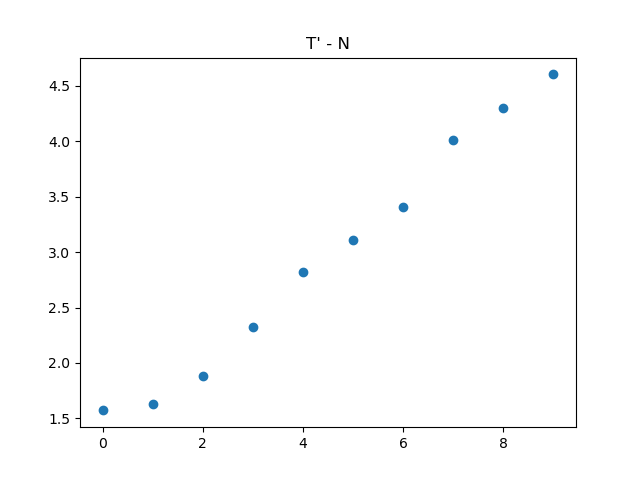
\includegraphics[height=2 in]{../pic/maxes.png }}
	\caption{The pictures I drew}
	\label{fig:maxes}
\end{figure}

Analyzing these digits, I found that with the same error $\epsilon$, if we raise the order of the $\hat{x}(t)$, the sampling rate can be set higher. In other words, it is the order of the reconstructed signal and the sampling rate decide the maximum of the error, and the two variables are negatively correlated when the error $\epsilon$ is fixed. So, if the accuracy is needed to be less, then what can be done is to raise the sampling rate or to raise the order of $\hat{x}(t)$.

\section{USB Hubs and My Proposal about It}
\subsection{USB Hubs}
The USB Hubs are those devices that expand one USB port to several other ports. Those ports are divided into two kinds, one is called upstream port (usually connected to PC) and the other is called the downstream ports (usually connected to I/O or storage devices).

The upstream port can access all the downstream ports. However, downstream ports cannot access any other ports except the upstream port. What's more, Time Division Multiplexing are applied to avoid the mess that all downstream ports transmit data at the same time.

Moreover, for a computer which is connected to the upstream port, if there's a device connected to the downstream ports, the computer will allocate an address to the newly connected device in order to manage and transmit data to it.

\subsection{My Proposal}




\section{Conclusion}
\subsubsection*{Videos}
I imagined how the stretch will work in a warehouse, and find an possible alternative of the suck disc stretches have.
\subsubsection*{Comparison Between Two Sampling Methods}
The differences of the two lie in
\begin{enumerate}
	\item Local Adaptivity
	\item Circuits
	\item Error
	\item Bandwidth
\end{enumerate}
\subsubsection*{USB Hubs and My Proposal about It}

\bibliographystyle{ieeetr}
\bibliography{../bib/database}

\begin{appendices}
\section{Code Listing}
\begin{python}
import numpy as np
from matplotlib import pyplot as plt

N = 10
t = np.arange(0, 20, 0.1)
func = np.cos(8*t)+np.sin(5*t)*np.cos(2*t)

fig1 = plt.figure()
plt.plot(t, func)
plt.show()

maxs = []
intv = [i for i in range(N)]

for i in range(1, N + 1):
    df = np.diff(func, i)
    df.resize(len(t))
    df /= (t[1] - t[0])**i
    nl = 1
    for j in range(1, i + 1):
        nl *= j
    maxs.append((nl/np.max(df))**(1/i))

fig2 = plt.figure()
plt.scatter(intv, maxs)
plt.show()
\end{python}
\end{appendices}

\end{document}